% Options for packages loaded elsewhere
\PassOptionsToPackage{unicode}{hyperref}
\PassOptionsToPackage{hyphens}{url}
%
\documentclass[
]{article}
\usepackage{amsmath,amssymb}
\usepackage{lmodern}
\usepackage{iftex}
\ifPDFTeX
  \usepackage[T1]{fontenc}
  \usepackage[utf8]{inputenc}
  \usepackage{textcomp} % provide euro and other symbols
\else % if luatex or xetex
  \usepackage{unicode-math}
  \defaultfontfeatures{Scale=MatchLowercase}
  \defaultfontfeatures[\rmfamily]{Ligatures=TeX,Scale=1}
\fi
% Use upquote if available, for straight quotes in verbatim environments
\IfFileExists{upquote.sty}{\usepackage{upquote}}{}
\IfFileExists{microtype.sty}{% use microtype if available
  \usepackage[]{microtype}
  \UseMicrotypeSet[protrusion]{basicmath} % disable protrusion for tt fonts
}{}
\makeatletter
\@ifundefined{KOMAClassName}{% if non-KOMA class
  \IfFileExists{parskip.sty}{%
    \usepackage{parskip}
  }{% else
    \setlength{\parindent}{0pt}
    \setlength{\parskip}{6pt plus 2pt minus 1pt}}
}{% if KOMA class
  \KOMAoptions{parskip=half}}
\makeatother
\usepackage{xcolor}
\usepackage[margin=1in]{geometry}
\usepackage{graphicx}
\makeatletter
\def\maxwidth{\ifdim\Gin@nat@width>\linewidth\linewidth\else\Gin@nat@width\fi}
\def\maxheight{\ifdim\Gin@nat@height>\textheight\textheight\else\Gin@nat@height\fi}
\makeatother
% Scale images if necessary, so that they will not overflow the page
% margins by default, and it is still possible to overwrite the defaults
% using explicit options in \includegraphics[width, height, ...]{}
\setkeys{Gin}{width=\maxwidth,height=\maxheight,keepaspectratio}
% Set default figure placement to htbp
\makeatletter
\def\fps@figure{htbp}
\makeatother
\setlength{\emergencystretch}{3em} % prevent overfull lines
\providecommand{\tightlist}{%
  \setlength{\itemsep}{0pt}\setlength{\parskip}{0pt}}
\setcounter{secnumdepth}{5}
\usepackage{booktabs,longtable,dcolumn} \usepackage{multirow,array} \usepackage{wrapfig,float} \floatplacement{figure}{H}
\ifLuaTeX
  \usepackage{selnolig}  % disable illegal ligatures
\fi
\IfFileExists{bookmark.sty}{\usepackage{bookmark}}{\usepackage{hyperref}}
\IfFileExists{xurl.sty}{\usepackage{xurl}}{} % add URL line breaks if available
\urlstyle{same} % disable monospaced font for URLs
\hypersetup{
  pdftitle={Percentage Delay Rate (with Time Independent Clean Control): QuickPay (2009-2012)},
  hidelinks,
  pdfcreator={LaTeX via pandoc}}

\title{Percentage Delay Rate (with Time Independent Clean Control):
QuickPay (2009-2012)}
\author{}
\date{\vspace{-2.5em}Feb 10, 2023}

\begin{document}
\maketitle

\begin{itemize}
\item
  Sample consists of a ``time independent'' clean control group

  \begin{itemize}
  \tightlist
  \item
    This means we keep all small projects.
  \item
    We keep only those large projects that don't have a concurrent small
    project in \emph{any} quarter.
  \end{itemize}
\item
  When we analyze congestion effect, we restrict to only one type of
  contractor. That is, contractors that hold only small project or only
  large project in the sample horizon.
\item
  Number of offers received is also winsorized.
\end{itemize}

\hypertarget{setup}{%
\section{Setup}\label{setup}}

\hypertarget{demeaned-delay-rate-in-percentage}{%
\section{Demeaned delay rate (in
percentage)}\label{demeaned-delay-rate-in-percentage}}

\begin{itemize}
\tightlist
\item
  Subtract the average pre-quickpay delay rate from each observation
\end{itemize}

\begin{verbatim}
## Warning: Using `size` aesthetic for lines was deprecated in ggplot2 3.4.0.
## i Please use `linewidth` instead.
\end{verbatim}

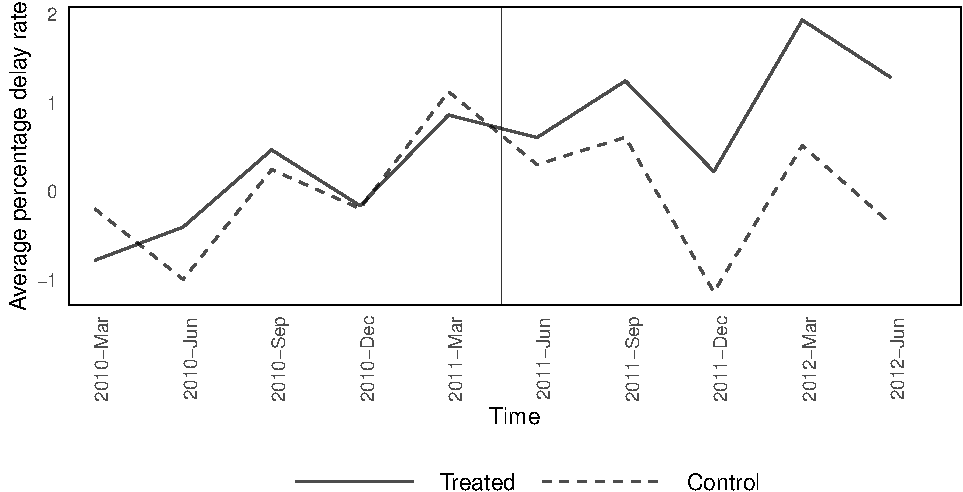
\includegraphics{qp_first_pc_delay_clean_control_time_independent_files/figure-latex/demeaned_plot_one_type-1.pdf}

\hypertarget{summary-statistics}{%
\section{Summary statistics}\label{summary-statistics}}

\begin{table}[ht]
\centering
\scalebox{0.75}{
\begin{tabular}{lrrrrrrrrrr}
  \toprule
Variable & SB.Mean & SB.Std Dev & SB.5\% & SB.95\% & SB.Obs & LB.Mean & LB.Std Dev & LB.5\% & LB.95\% & LB.Obs \\ 
  \midrule
Percentage delay & 3.88 & 25.08 & 0.00 & 14.07 & 45944 & 5.69 & 30.93 & 0.00 & 33.59 & 35894 \\ 
  Initial duration (in days) & 256.25 & 155.34 & 76.00 & 489.00 & 45944 & 282.14 & 163.94 & 80.00 & 568.00 & 35894 \\ 
  Initial budget (000s) & 534.94 & 2338.67 & 3.31 & 2535.99 & 45944 & 1440.09 & 5164.52 & 3.71 & 7492.45 & 35894 \\ 
  Number of offers & 4.58 & 6.59 & 1.00 & 15.00 & 45944 & 3.96 & 9.30 & 1.00 & 13.00 & 35894 \\ 
  Project stage & 0.33 & 0.23 & 0.02 & 0.75 & 45944 & 0.34 & 0.24 & 0.02 & 0.75 & 35894 \\ 
  Positive delay (indicator) & 0.06 & 0.24 & 0.00 & 1.00 & 45944 & 0.08 & 0.28 & 0.00 & 1.00 & 35894 \\ 
  Negative delay (indicator) & 0.01 & 0.09 & 0.00 & 0.00 & 45944 & 0.01 & 0.09 & 0.00 & 0.00 & 35894 \\ 
  Competitively awarded (indicator) & 0.87 & 0.33 & 0.00 & 1.00 & 45944 & 0.81 & 0.39 & 0.00 & 1.00 & 35894 \\ 
  Contract financing (indicator) & 0.13 & 0.33 & 0.00 & 1.00 & 45944 & 0.14 & 0.34 & 0.00 & 1.00 & 35894 \\ 
   \bottomrule
\end{tabular}
}
\caption{Before QuickPay} 
\end{table}
\begin{table}[ht]
\centering
\scalebox{0.75}{
\begin{tabular}{lrrrrrrrrrr}
  \toprule
Variable & SB.Mean & SB.Std Dev & SB.5\% & SB.95\% & SB.Obs & LB.Mean & LB.Std Dev & LB.5\% & LB.95\% & LB.Obs \\ 
  \midrule
Percentage delay & 4.36 & 23.32 & 0.00 & 27.22 & 67523 & 4.54 & 24.02 & 0.00 & 29.59 & 60748 \\ 
  Initial duration (in days) & 293.29 & 179.56 & 87.00 & 606.00 & 67523 & 337.92 & 199.09 & 90.00 & 733.00 & 60748 \\ 
  Initial budget (000s) & 750.96 & 2911.52 & 3.51 & 3886.88 & 67523 & 1824.54 & 6141.86 & 3.72 & 10306.48 & 60748 \\ 
  Number of offers & 4.62 & 5.60 & 1.00 & 15.00 & 67523 & 3.67 & 7.12 & 1.00 & 12.00 & 60748 \\ 
  Project stage & 0.41 & 0.26 & 0.03 & 0.85 & 67523 & 0.43 & 0.26 & 0.03 & 0.85 & 60748 \\ 
  Positive delay (indicator) & 0.09 & 0.28 & 0.00 & 1.00 & 67523 & 0.10 & 0.29 & 0.00 & 1.00 & 60748 \\ 
  Negative delay (indicator) & 0.01 & 0.08 & 0.00 & 0.00 & 67523 & 0.01 & 0.10 & 0.00 & 0.00 & 60748 \\ 
  Competitively awarded (indicator) & 0.87 & 0.34 & 0.00 & 1.00 & 67523 & 0.72 & 0.45 & 0.00 & 1.00 & 60748 \\ 
  Contract financing (indicator) & 0.13 & 0.33 & 0.00 & 1.00 & 67523 & 0.14 & 0.35 & 0.00 & 1.00 & 60748 \\ 
   \bottomrule
\end{tabular}
}
\caption{After QuickPay} 
\end{table}
\begin{table}[ht]
\centering
\scalebox{0.75}{
\begin{tabular}{lrrrr}
  \toprule
var\_name & SB.before & LB.before & SB.after & LB.after \\ 
  \midrule
Number of tasks & 786 & 707 & 947 & 947 \\ 
  Number of industries & 64 & 65 & 62 & 62 \\ 
   \bottomrule
\end{tabular}
}
\end{table}

\hypertarget{baseline-regressions}{%
\section{Baseline Regressions}\label{baseline-regressions}}

\[ PercentDelay_{it} = \beta_0 + \beta_1 Treat_i + \beta_2 Post_t + \beta_3 (Treat_i \times Post_t) + e_{it}\]

\[ \begin{aligned} PercentDelay_{it} &=& \alpha+\beta_0 Treat_i + \beta_1 Post_t + \beta_2 (Treat_i \times Post_t)\\
&+&  X_i + (Post_t \times X_i) + \mu_t + \theta_{firm} + \lambda_{task}+ \epsilon_{it}
\end{aligned}\]

\begin{table}[H] \centering 
  \caption{Effect of QuickPay on project delay rates} 
  \label{} 
\small 
\begin{tabular}{@{\extracolsep{-2pt}}lccccc} 
\\[-1.8ex]\hline 
\hline \\[-1.8ex] 
\\[-1.8ex] & \multicolumn{5}{c}{$PercentDelay_{it}$} \\ 
\\[-1.8ex] & (1) & (2) & (3) & (4) & (5)\\ 
\hline \\[-1.8ex] 
 $Treat_i$ & $-$1.76$^{***}$ & $-$1.30$^{***}$ & $-$1.35$^{***}$ & $-$0.90$^{***}$ & $-$0.91$^{***}$ \\ 
  & (0.11) & (0.11) & (0.11) & (0.11) & (0.11) \\ 
  & & & & & \\ 
 $Post_t$ & $-$0.21$^{*}$ & $-$5.57$^{***}$ &  &  &  \\ 
  & (0.12) & (0.78) &  &  &  \\ 
  & & & & & \\ 
 $Treat_i \times Post_t$ & 1.10$^{***}$ & 0.97$^{***}$ & 1.01$^{***}$ & 0.99$^{***}$ & 1.01$^{***}$ \\ 
  & (0.14) & (0.14) & (0.14) & (0.13) & (0.13) \\ 
  & & & & & \\ 
 Constant & 5.27$^{***}$ & 43.19$^{***}$ &  &  &  \\ 
  & (0.10) & (0.61) &  &  &  \\ 
  & & & & & \\ 
\hline \\[-1.8ex] 
Duration, Budget, Bids & No & Yes & Yes & Yes & Yes \\ 
$Post_t \times$  (Duration, Budget, Bids) & No & Yes & Yes & Yes & Yes \\ 
Project stage & No & Yes & Yes & Yes & Yes \\ 
Time fixed effects & No & No & Yes & Yes & Yes \\ 
Task fixed effects & No & No & No & Yes & Yes \\ 
Industry fixed effects & No & No & No & No & Yes \\ 
Observations & 223,244 & 201,738 & 201,738 & 201,738 & 201,738 \\ 
R$^{2}$ & 0.002 & 0.17 & 0.18 & 0.21 & 0.21 \\ 
Adjusted R$^{2}$ & 0.002 & 0.17 & 0.18 & 0.21 & 0.21 \\ 
\hline 
\hline \\[-1.8ex] 
\textit{Note:}  & \multicolumn{5}{r}{$^{*}$p$<$0.1; $^{**}$p$<$0.05; $^{***}$p$<$0.01} \\ 
 & \multicolumn{5}{r}{Each observation is a project-quarter.} \\ 
 & \multicolumn{5}{r}{SEs are robust and clustered at the project level.} \\ 
\end{tabular} 
\end{table}

\hypertarget{days-of-delay-one-quarter}{%
\section{Days of delay (One Quarter)}\label{days-of-delay-one-quarter}}

\begin{table}[H] \centering 
  \caption{Effect of QuickPay on project delay rates} 
  \label{} 
\small 
\begin{tabular}{@{\extracolsep{-2pt}}lccccc} 
\\[-1.8ex]\hline 
\hline \\[-1.8ex] 
\\[-1.8ex] & \multicolumn{5}{c}{$DelayDays_{it}$} \\ 
\\[-1.8ex] & (1) & (2) & (3) & (4) & (5)\\ 
\hline \\[-1.8ex] 
 $Treat_i$ & $-$3.44$^{***}$ & $-$2.28$^{***}$ & $-$2.38$^{***}$ & $-$1.81$^{***}$ & $-$1.84$^{***}$ \\ 
  & (0.19) & (0.18) & (0.18) & (0.18) & (0.18) \\ 
  & & & & & \\ 
 $Post_t$ & 1.24$^{***}$ & $-$5.79$^{***}$ &  &  &  \\ 
  & (0.20) & (1.23) &  &  &  \\ 
  & & & & & \\ 
 $Treat_i \times Post_t$ & 1.51$^{***}$ & 1.69$^{***}$ & 1.78$^{***}$ & 1.72$^{***}$ & 1.74$^{***}$ \\ 
  & (0.24) & (0.24) & (0.24) & (0.24) & (0.24) \\ 
  & & & & & \\ 
 Constant & 8.80$^{***}$ & 53.07$^{***}$ &  &  &  \\ 
  & (0.16) & (0.92) &  &  &  \\ 
  & & & & & \\ 
\hline \\[-1.8ex] 
Duration, Budget, Bids & No & Yes & Yes & Yes & Yes \\ 
$Post_t \times$  (Duration, Budget, Bids) & No & Yes & Yes & Yes & Yes \\ 
Project stage & No & Yes & Yes & Yes & Yes \\ 
Time fixed effects & No & No & Yes & Yes & Yes \\ 
Task fixed effects & No & No & No & Yes & Yes \\ 
Industry fixed effects & No & No & No & No & Yes \\ 
Observations & 223,373 & 201,867 & 201,867 & 201,867 & 201,867 \\ 
R$^{2}$ & 0.004 & 0.14 & 0.14 & 0.18 & 0.18 \\ 
Adjusted R$^{2}$ & 0.004 & 0.14 & 0.14 & 0.17 & 0.17 \\ 
\hline 
\hline \\[-1.8ex] 
\textit{Note:}  & \multicolumn{5}{r}{$^{*}$p$<$0.1; $^{**}$p$<$0.05; $^{***}$p$<$0.01} \\ 
 & \multicolumn{5}{r}{Each observation is a project-quarter.} \\ 
 & \multicolumn{5}{r}{SEs are robust and clustered at the project level.} \\ 
\end{tabular} 
\end{table}

\hypertarget{days-of-delay-two-quarters}{%
\section{Days of delay (Two
Quarters)}\label{days-of-delay-two-quarters}}

\begin{table}[H] \centering 
  \caption{Effect of QuickPay on project delay rates} 
  \label{} 
\small 
\begin{tabular}{@{\extracolsep{-2pt}}lccccc} 
\\[-1.8ex]\hline 
\hline \\[-1.8ex] 
\\[-1.8ex] & \multicolumn{5}{c}{$DelayRate_{it}$} \\ 
\\[-1.8ex] & (1) & (2) & (3) & (4) & (5)\\ 
\hline \\[-1.8ex] 
 $Treat_i$ & $-$8.52$^{***}$ & $-$5.20$^{***}$ & $-$5.37$^{***}$ & $-$3.93$^{***}$ & $-$3.77$^{***}$ \\ 
  & (0.52) & (0.53) & (0.53) & (0.55) & (0.55) \\ 
  & & & & & \\ 
 $Post_t$ & 4.43$^{***}$ & $-$18.77$^{***}$ &  &  &  \\ 
  & (0.59) & (3.66) &  &  &  \\ 
  & & & & & \\ 
 $Treat_i \times Post_t$ & 3.17$^{***}$ & 3.58$^{***}$ & 3.75$^{***}$ & 3.89$^{***}$ & 3.87$^{***}$ \\ 
  & (0.70) & (0.73) & (0.73) & (0.74) & (0.74) \\ 
  & & & & & \\ 
 Constant & 21.06$^{***}$ & 116.48$^{***}$ &  &  &  \\ 
  & (0.45) & (2.67) &  &  &  \\ 
  & & & & & \\ 
\hline \\[-1.8ex] 
Duration, Budget, Bids & No & Yes & Yes & Yes & Yes \\ 
$Post_t \times$  (Duration, Budget, Bids) & No & Yes & Yes & Yes & Yes \\ 
Project stage & No & Yes & Yes & Yes & Yes \\ 
Year-Quarter fixed effects & No & No & Yes & Yes & Yes \\ 
Task fixed effects & No & No & No & Yes & Yes \\ 
Industry fixed effects & No & No & No & No & Yes \\ 
Observations & 94,123 & 84,737 & 84,737 & 84,737 & 84,737 \\ 
R$^{2}$ & 0.01 & 0.17 & 0.17 & 0.22 & 0.22 \\ 
Adjusted R$^{2}$ & 0.01 & 0.17 & 0.17 & 0.20 & 0.21 \\ 
\hline 
\hline \\[-1.8ex] 
\textit{Note:}  & \multicolumn{5}{r}{$^{*}$p$<$0.1; $^{**}$p$<$0.05; $^{***}$p$<$0.01} \\ 
 & \multicolumn{5}{r}{SEs are robust and clustered at the project level.} \\ 
\end{tabular} 
\end{table}

\hypertarget{positive-delays-logit}{%
\section{Positive delays: Logit}\label{positive-delays-logit}}

\begin{table}[htbp]
   \caption{Logit model: Effect of QuickPay}
   \centering
   \begin{tabular}{lccccc}
      \tabularnewline \midrule \midrule
      Dependent Variable: & \multicolumn{5}{c}{$I(Delay_{it}>0)$}\\
      Model:                       & (1)           & (2)           & (3)           & (4)           & (5)\\  
      \midrule
      \emph{Variables}\\
      Constant                     & -1.99$^{***}$ & 3.22$^{***}$  &               &               &   \\   
                                   & (0.02)        & (0.13)        &               &               &   \\   
      $Treat_i$                    & -0.44$^{***}$ & -0.22$^{***}$ & -0.24$^{***}$ & -0.21$^{***}$ & -0.23$^{***}$\\   
                                   & (0.03)        & (0.03)        & (0.03)        & (0.03)        & (0.03)\\   
      $Post_t$                     & 0.10$^{***}$  & -1.42$^{***}$ &               &               &   \\   
                                   & (0.02)        & (0.15)        &               &               &   \\   
      $Treat_i$ $\times$ $Post_t$  & 0.21$^{***}$  & 0.21$^{***}$  & 0.23$^{***}$  & 0.23$^{***}$  & 0.23$^{***}$\\   
                                   & (0.03)        & (0.04)        & (0.04)        & (0.04)        & (0.04)\\   
      Controls                     &               & Yes           & Yes           & Yes           & Yes\\  
      Controls $\times Post_t$     &               & Yes           & Yes           & Yes           & Yes\\  
      \midrule
      \emph{Fixed-effects}\\
      Time                         &               &               & Yes           & Yes           & Yes\\  
      Task code                    &               &               &               & Yes           & Yes\\  
      NAICS code                   &               &               &               &               & Yes\\  
      \midrule
      \emph{Fit statistics}\\
      Observations                 & 223,373       & 201,867       & 201,867       & 199,508       & 199,470\\  
      Squared Correlation          & 0.003         & 0.24          & 0.24          & 0.28          & 0.28\\  
      Pseudo R$^2$                 & 0.005         & 0.24          & 0.24          & 0.30          & 0.30\\  
      BIC                          & 152,027.7     & 112,255.0     & 112,164.9     & 113,713.7     & 113,928.5\\  
      \midrule \midrule
      \multicolumn{6}{l}{\emph{Clustered (Project ID) standard-errors in parentheses}}\\
      \multicolumn{6}{l}{\emph{Signif. Codes: ***: 0.01, **: 0.05, *: 0.1}}\\
   \end{tabular}
\end{table}

\hypertarget{positive-delays-conditional-te}{%
\section{Positive delays: Conditional
TE}\label{positive-delays-conditional-te}}

\begin{table}[H] \centering 
  \caption{Conditional TE: Positive delay} 
  \label{} 
\small 
\begin{tabular}{@{\extracolsep{-2pt}}lccccc} 
\\[-1.8ex]\hline 
\hline \\[-1.8ex] 
\\[-1.8ex] & \multicolumn{5}{c}{$PercentDelay_{it} (conditional on positive)$} \\ 
\\[-1.8ex] & (1) & (2) & (3) & (4) & (5)\\ 
\hline \\[-1.8ex] 
 $Treat_i$ & $-$5.87 & $-$22.68$^{***}$ & $-$22.85$^{***}$ & $-$25.17$^{***}$ & $-$25.24$^{***}$ \\ 
  & (5.42) & (4.28) & (4.28) & (4.59) & (4.64) \\ 
  & & & & & \\ 
 $Post_t$ & $-$51.73$^{***}$ & $-$36.01$^{*}$ &  &  &  \\ 
  & (4.68) & (19.74) &  &  &  \\ 
  & & & & & \\ 
 $Treat_i \times Post_t$ & 15.61$^{**}$ & 22.58$^{***}$ & 22.77$^{***}$ & 26.76$^{***}$ & 28.25$^{***}$ \\ 
  & (6.20) & (4.98) & (4.99) & (5.03) & (5.03) \\ 
  & & & & & \\ 
 Constant & 160.76$^{***}$ & 694.17$^{***}$ &  &  &  \\ 
  & (4.08) & (15.55) &  &  &  \\ 
  & & & & & \\ 
\hline \\[-1.8ex] 
Duration, Budget, Bids & No & Yes & Yes & Yes & Yes \\ 
$Post_t \times$  (Duration, Budget, Bids) & No & Yes & Yes & Yes & Yes \\ 
Project stage & No & Yes & Yes & Yes & Yes \\ 
Time fixed effects & No & No & Yes & Yes & Yes \\ 
Task fixed effects & No & No & No & Yes & Yes \\ 
Industry fixed effects & No & No & No & No & Yes \\ 
Observations & 24,084 & 24,045 & 24,045 & 24,045 & 24,045 \\ 
R$^{2}$ & 0.01 & 0.39 & 0.39 & 0.46 & 0.47 \\ 
Adjusted R$^{2}$ & 0.01 & 0.39 & 0.39 & 0.44 & 0.45 \\ 
\hline 
\hline \\[-1.8ex] 
\textit{Note:}  & \multicolumn{5}{r}{$^{*}$p$<$0.1; $^{**}$p$<$0.05; $^{***}$p$<$0.01} \\ 
 & \multicolumn{5}{r}{Each observation is a project-quarter.} \\ 
 & \multicolumn{5}{r}{SEs are robust and clustered at the project level.} \\ 
\end{tabular} 
\end{table}

\hypertarget{negative-delays-logit}{%
\section{Negative delays: Logit}\label{negative-delays-logit}}

\begin{table}[htbp]
   \caption{Logit model: Effect of QuickPay}
   \centering
   \begin{tabular}{lccccc}
      \tabularnewline \midrule \midrule
      Dependent Variable: & \multicolumn{5}{c}{$I(Delay_{it}<0)$}\\
      Model:                       & (1)           & (2)            & (3)           & (4)           & (5)\\  
      \midrule
      \emph{Variables}\\
      Constant                     & -4.61$^{***}$ & -10.07$^{***}$ &               &               &   \\   
                                   & (0.06)        & (0.44)         &               &               &   \\   
      $Treat_i$                    & -0.29$^{***}$ & 0.13           & 0.14$^{*}$    & 0.02          & 0.02\\   
                                   & (0.08)        & (0.09)         & (0.09)        & (0.09)        & (0.09)\\   
      $Post_t$                     & 0.07          & 1.50$^{***}$   &               &               &   \\   
                                   & (0.07)        & (0.56)         &               &               &   \\   
      $Treat_i$ $\times$ $Post_t$  & -0.24$^{**}$  & -0.31$^{***}$  & -0.32$^{***}$ & -0.29$^{***}$ & -0.29$^{***}$\\   
                                   & (0.10)        & (0.11)         & (0.11)        & (0.10)        & (0.10)\\   
      Controls                     &               & Yes            & Yes           & Yes           & Yes\\  
      Controls $\times Post_t$     &               & Yes            & Yes           & Yes           & Yes\\  
      \midrule
      \emph{Fixed-effects}\\
      Time                         &               &                & Yes           & Yes           & Yes\\  
      Task code                    &               &                &               & Yes           & Yes\\  
      NAICS code                   &               &                &               &               & Yes\\  
      \midrule
      \emph{Fit statistics}\\
      Observations                 & 223,373       & 201,867        & 201,867       & 177,464       & 176,917\\  
      Squared Correlation          & 0.0004        & 0.007          & 0.008         & 0.02          & 0.03\\  
      Pseudo R$^2$                 & 0.004         & 0.05           & 0.06          & 0.12          & 0.12\\  
      BIC                          & 20,766.4      & 19,492.5       & 19,549.3      & 21,853.5      & 22,368.3\\  
      \midrule \midrule
      \multicolumn{6}{l}{\emph{Clustered (Project ID) standard-errors in parentheses}}\\
      \multicolumn{6}{l}{\emph{Signif. Codes: ***: 0.01, **: 0.05, *: 0.1}}\\
   \end{tabular}
\end{table}

\hypertarget{negative-delays-conditional-te}{%
\section{Negative delays: Conditional
TE}\label{negative-delays-conditional-te}}

\begin{table}[H] \centering 
  \caption{Conditional TE: Negative delay (conditional on negative)} 
  \label{} 
\small 
\begin{tabular}{@{\extracolsep{-2pt}}lccccc} 
\\[-1.8ex]\hline 
\hline \\[-1.8ex] 
\\[-1.8ex] & \multicolumn{5}{c}{$PercentDelay_{it}$} \\ 
\\[-1.8ex] & (1) & (2) & (3) & (4) & (5)\\ 
\hline \\[-1.8ex] 
 $Treat_i$ & 3.72$^{*}$ & 2.28 & 2.27 & 0.74 & 1.06 \\ 
  & (2.15) & (1.98) & (2.00) & (2.43) & (2.47) \\ 
  & & & & & \\ 
 $Post_t$ & 8.13$^{***}$ & $-$2.26 &  &  &  \\ 
  & (2.01) & (9.66) &  &  &  \\ 
  & & & & & \\ 
 $Treat_i \times Post_t$ & $-$8.74$^{***}$ & $-$5.62$^{**}$ & $-$5.44$^{**}$ & $-$2.87 & $-$3.55 \\ 
  & (2.72) & (2.47) & (2.48) & (3.00) & (3.03) \\ 
  & & & & & \\ 
 Constant & $-$35.47$^{***}$ & 7.39 &  &  &  \\ 
  & (1.66) & (8.06) &  &  &  \\ 
  & & & & & \\ 
\hline \\[-1.8ex] 
Duration, Budget, Bids & No & Yes & Yes & Yes & Yes \\ 
$Post_t \times$  (Duration, Budget, Bids) & No & Yes & Yes & Yes & Yes \\ 
Project stage & No & Yes & Yes & Yes & Yes \\ 
Time fixed effects & No & No & Yes & Yes & Yes \\ 
Task fixed effects & No & No & No & Yes & Yes \\ 
Industry fixed effects & No & No & No & No & Yes \\ 
Observations & 1,786 & 1,786 & 1,786 & 1,786 & 1,786 \\ 
R$^{2}$ & 0.01 & 0.22 & 0.23 & 0.39 & 0.43 \\ 
Adjusted R$^{2}$ & 0.01 & 0.22 & 0.22 & 0.24 & 0.27 \\ 
\hline 
\hline \\[-1.8ex] 
\textit{Note:}  & \multicolumn{5}{r}{$^{*}$p$<$0.1; $^{**}$p$<$0.05; $^{***}$p$<$0.01} \\ 
 & \multicolumn{5}{r}{Each observation is a project-quarter.} \\ 
 & \multicolumn{5}{r}{SEs are robust and clustered at the project level.} \\ 
\end{tabular} 
\end{table}

\hypertarget{event-study}{%
\section{Event study}\label{event-study}}

\(PercentDelay_{it}=\beta_0 + \beta_1 Treat_i + \beta_2 Treat_i \times Quarter_t + Controls + \gamma_{task} + \theta_{naics}+\lambda_{quarter}+\epsilon_{it}\)

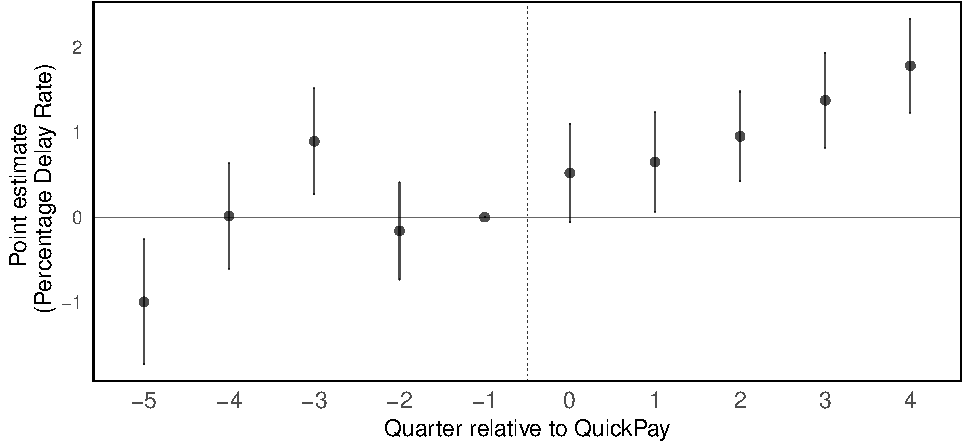
\includegraphics{qp_first_pc_delay_clean_control_time_independent_files/figure-latex/event_study-1.pdf}

\hypertarget{parallel-trends-test}{%
\section{Parallel Trends Test}\label{parallel-trends-test}}

\begin{table}[H] \centering 
  \caption{Linear Time Trend Before QuickPay} 
  \label{} 
\small 
\begin{tabular}{@{\extracolsep{-2pt}}lccccc} 
\\[-1.8ex]\hline 
\hline \\[-1.8ex] 
\\[-1.8ex] & \multicolumn{5}{c}{$PercentDelay_{it}$} \\ 
\\[-1.8ex] & (1) & (2) & (3) & (4) & (5)\\ 
\hline \\[-1.8ex] 
 $Treat_i$ & $-$1.37$^{***}$ & $-$0.65 & $-$0.65 & $-$0.44 & $-$0.52 \\ 
  & (0.41) & (0.41) & (0.41) & (0.41) & (0.41) \\ 
  & & & & & \\ 
 $QuarterNum$ & 0.42$^{***}$ & $-$1.16$^{**}$ &  &  &  \\ 
  & (0.08) & (0.50) &  &  &  \\ 
  & & & & & \\ 
 $Treat_i \times QuarterNum$ & $-$0.09 & $-$0.17$^{*}$ & $-$0.17$^{*}$ & $-$0.03 & $-$0.03 \\ 
  & (0.09) & (0.09) & (0.09) & (0.09) & (0.09) \\ 
  & & & & & \\ 
 Constant & 3.36$^{***}$ & 48.76$^{***}$ &  &  &  \\ 
  & (0.35) & (2.32) &  &  &  \\ 
  & & & & & \\ 
\hline \\[-1.8ex] 
Duration, Budget, Bids & No & Yes & Yes & Yes & Yes \\ 
$Post_t \times$  (Duration, Budget, Bids) & No & Yes & Yes & Yes & Yes \\ 
Project stage & No & Yes & Yes & Yes & Yes \\ 
Time fixed effects & No & No & Yes & Yes & Yes \\ 
Task fixed effects & No & No & No & Yes & Yes \\ 
Industry fixed effects & No & No & No & No & Yes \\ 
Observations & 84,367 & 77,984 & 77,984 & 77,984 & 77,984 \\ 
R$^{2}$ & 0.005 & 0.20 & 0.20 & 0.26 & 0.27 \\ 
Adjusted R$^{2}$ & 0.005 & 0.20 & 0.20 & 0.25 & 0.26 \\ 
\hline 
\hline \\[-1.8ex] 
\textit{Note:}  & \multicolumn{5}{r}{$^{*}$p$<$0.1; $^{**}$p$<$0.05; $^{***}$p$<$0.01} \\ 
 & \multicolumn{5}{r}{Each observation is a project-quarter.} \\ 
 & \multicolumn{5}{r}{SEs are robust and clustered at the project level.} \\ 
 & \multicolumn{5}{r}{Observations are for quarters before quickpay.} \\ 
\end{tabular} 
\end{table}

\hypertarget{temporal-placebo-test}{%
\section{Temporal Placebo Test}\label{temporal-placebo-test}}

\begin{itemize}
\tightlist
\item
  Restrict to pre-QuickPay observations
\item
  Assign ``treatment date'' as 2010-09-30
\end{itemize}

{[}1{]} 4

\begin{table}[H] \centering 
  \caption{Placebo test: Treatment Time 2010-09-30} 
  \label{} 
\small 
\begin{tabular}{@{\extracolsep{-2pt}}lccccc} 
\\[-1.8ex]\hline 
\hline \\[-1.8ex] 
\\[-1.8ex] & \multicolumn{5}{c}{$PercentDelay_{it}$} \\ 
\\[-1.8ex] & (1) & (2) & (3) & (4) & (5)\\ 
\hline \\[-1.8ex] 
 $Treat_i$ & $-$1.62$^{***}$ & $-$1.56$^{***}$ & $-$1.57$^{***}$ & $-$0.80$^{***}$ & $-$0.85$^{***}$ \\ 
  & (0.22) & (0.22) & (0.22) & (0.22) & (0.22) \\ 
  & & & & & \\ 
 $Post$ & 1.12$^{***}$ & $-$5.03$^{***}$ &  &  &  \\ 
  & (0.21) & (1.50) &  &  &  \\ 
  & & & & & \\ 
 $Treat_i \times Post$ & $-$0.20 & 0.23 & 0.23 & 0.31 & 0.32 \\ 
  & (0.25) & (0.25) & (0.25) & (0.25) & (0.25) \\ 
  & & & & & \\ 
 Constant & 4.45$^{***}$ & 48.36$^{***}$ &  &  &  \\ 
  & (0.19) & (1.30) &  &  &  \\ 
  & & & & & \\ 
\hline \\[-1.8ex] 
Duration, Budget, Bids & No & Yes & Yes & Yes & Yes \\ 
$Post_t \times$  (Duration, Budget, Bids) & No & Yes & Yes & Yes & Yes \\ 
Project stage & No & Yes & Yes & Yes & Yes \\ 
Time fixed effects & No & No & Yes & Yes & Yes \\ 
Task fixed effects & No & No & No & Yes & Yes \\ 
Industry fixed effects & No & No & No & No & Yes \\ 
Observations & 84,367 & 77,984 & 77,984 & 77,984 & 77,984 \\ 
R$^{2}$ & 0.004 & 0.20 & 0.20 & 0.26 & 0.27 \\ 
Adjusted R$^{2}$ & 0.004 & 0.20 & 0.20 & 0.25 & 0.26 \\ 
\hline 
\hline \\[-1.8ex] 
\textit{Note:}  & \multicolumn{5}{r}{$^{*}$p$<$0.1; $^{**}$p$<$0.05; $^{***}$p$<$0.01} \\ 
 & \multicolumn{5}{r}{Each observation is a project-quarter.} \\ 
 & \multicolumn{5}{r}{SEs are robust and clustered at the project level.} \\ 
 & \multicolumn{5}{r}{Observations are for quarters before quickpay.} \\ 
\end{tabular} 
\end{table}

\hypertarget{cross-sectional-placebo}{%
\section{Cross-sectional placebo}\label{cross-sectional-placebo}}

\begin{itemize}
\tightlist
\item
  Projects are randomly assigned into treatment or control
\end{itemize}

\begin{table}[H] \centering 
  \caption{Effect of QuickPay on project delay rates} 
  \label{} 
\small 
\begin{tabular}{@{\extracolsep{-2pt}}lccccc} 
\\[-1.8ex]\hline 
\hline \\[-1.8ex] 
\\[-1.8ex] & \multicolumn{5}{c}{$PercentDelay_{it}$} \\ 
\\[-1.8ex] & (1) & (2) & (3) & (4) & (5)\\ 
\hline \\[-1.8ex] 
 $Treat_i$ & $-$0.04 & $-$0.10 & $-$0.10 & $-$0.07 & $-$0.07 \\ 
  & (0.10) & (0.09) & (0.09) & (0.09) & (0.09) \\ 
  & & & & & \\ 
 $Post_t$ & 0.52$^{***}$ & $-$4.41$^{***}$ &  &  &  \\ 
  & (0.09) & (0.75) &  &  &  \\ 
  & & & & & \\ 
 $Treat_i \times Post_t$ & 0.02 & 0.02 & 0.02 & 0.03 & 0.03 \\ 
  & (0.13) & (0.12) & (0.12) & (0.11) & (0.11) \\ 
  & & & & & \\ 
 Constant & 4.14$^{***}$ & 41.68$^{***}$ &  &  &  \\ 
  & (0.07) & (0.58) &  &  &  \\ 
  & & & & & \\ 
\hline \\[-1.8ex] 
Duration, Budget, Bids & No & Yes & Yes & Yes & Yes \\ 
$Post_t \times$  (Duration, Budget, Bids) & No & Yes & Yes & Yes & Yes \\ 
Project stage & No & Yes & Yes & Yes & Yes \\ 
Time fixed effects & No & No & Yes & Yes & Yes \\ 
Task fixed effects & No & No & No & Yes & Yes \\ 
Industry fixed effects & No & No & No & No & Yes \\ 
Observations & 223,244 & 201,738 & 201,738 & 201,738 & 201,738 \\ 
R$^{2}$ & 0.0003 & 0.17 & 0.17 & 0.21 & 0.21 \\ 
Adjusted R$^{2}$ & 0.0003 & 0.17 & 0.17 & 0.21 & 0.21 \\ 
\hline 
\hline \\[-1.8ex] 
\textit{Note:}  & \multicolumn{5}{r}{$^{*}$p$<$0.1; $^{**}$p$<$0.05; $^{***}$p$<$0.01} \\ 
 & \multicolumn{5}{r}{Each observation is a project-quarter.} \\ 
 & \multicolumn{5}{r}{SEs are robust and clustered at the project level.} \\ 
\end{tabular} 
\end{table}

\hypertarget{congestion-effect}{%
\section{Congestion Effect}\label{congestion-effect}}

\hypertarget{number-of-projects-per-contractor}{%
\subsection{Number of projects per
contractor}\label{number-of-projects-per-contractor}}

\hypertarget{contractors-holding-only-small-or-only-large-projects}{%
\subsubsection{Contractors holding only small or only large
projects}\label{contractors-holding-only-small-or-only-large-projects}}

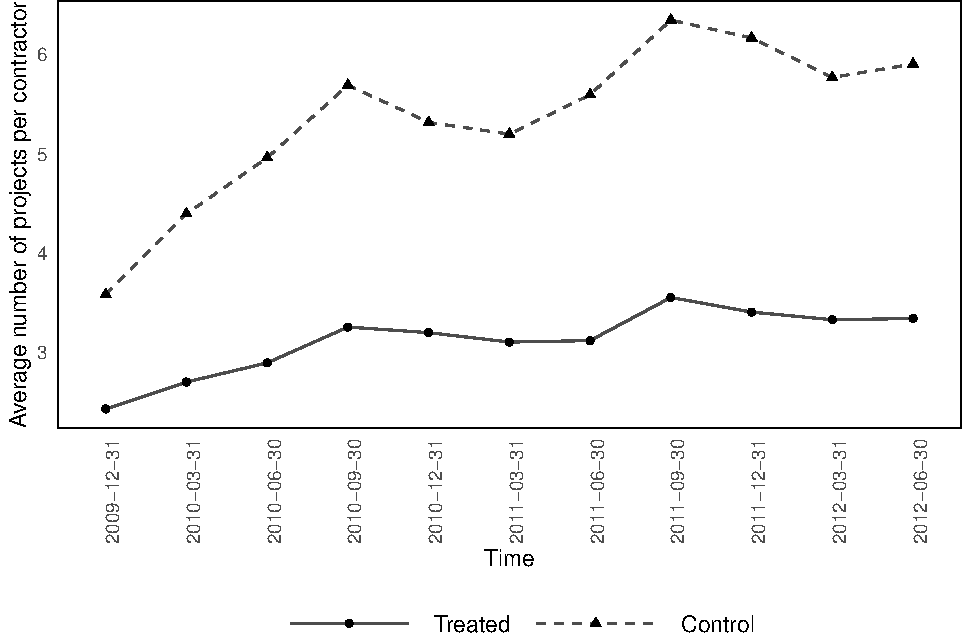
\includegraphics{qp_first_pc_delay_clean_control_time_independent_files/figure-latex/num_projects_0-1.pdf}

\begin{table}[H] \centering 
  \caption{Num Contractor Projects and QuickPay reform} 
  \label{} 
\small 
\begin{tabular}{@{\extracolsep{-2pt}}lcc} 
\\[-1.8ex]\hline 
\hline \\[-1.8ex] 
\\[-1.8ex] & \multicolumn{2}{c}{Number of projects} \\ 
\\[-1.8ex] & (1) & (2)\\ 
\hline \\[-1.8ex] 
 $Treat_i$ & $-$2.03$^{***}$ & $-$2.03$^{***}$ \\ 
  & (0.39) & (0.39) \\ 
  & & \\ 
 $Post_t$ & 0.94$^{**}$ &  \\ 
  & (0.41) &  \\ 
  & & \\ 
 $Treat_i \times Post_t$ & $-$0.58 & $-$0.58 \\ 
  & (0.41) & (0.41) \\ 
  & & \\ 
 Constant & 5.03$^{***}$ &  \\ 
  & (0.38) &  \\ 
  & & \\ 
\hline \\[-1.8ex] 
Time fixed effects & No & Yes \\ 
Observations & 84,391 & 84,391 \\ 
R$^{2}$ & 0.005 & 0.01 \\ 
Adjusted R$^{2}$ & 0.005 & 0.01 \\ 
\hline 
\hline \\[-1.8ex] 
\textit{Note:}  & \multicolumn{2}{r}{$^{*}$p$<$0.1; $^{**}$p$<$0.05; $^{***}$p$<$0.01} \\ 
 & \multicolumn{2}{r}{Each observation is a contractor-quarter.} \\ 
 & \multicolumn{2}{r}{SEs are robust and clustered at the contractor level.} \\ 
 & \multicolumn{2}{r}{Sample restricted to contractors performing only one type of project.} \\ 
\end{tabular} 
\end{table}

\hypertarget{contractors-holding-at-least-one-small-project-are-treated}{%
\subsubsection{Contractors holding at least one small project are
``treated''}\label{contractors-holding-at-least-one-small-project-are-treated}}

\hypertarget{total-budget}{%
\subsection{Total budget}\label{total-budget}}

\hypertarget{contractors-holding-only-small-or-only-large-projects-1}{%
\subsubsection{Contractors holding only small or only large
projects}\label{contractors-holding-only-small-or-only-large-projects-1}}

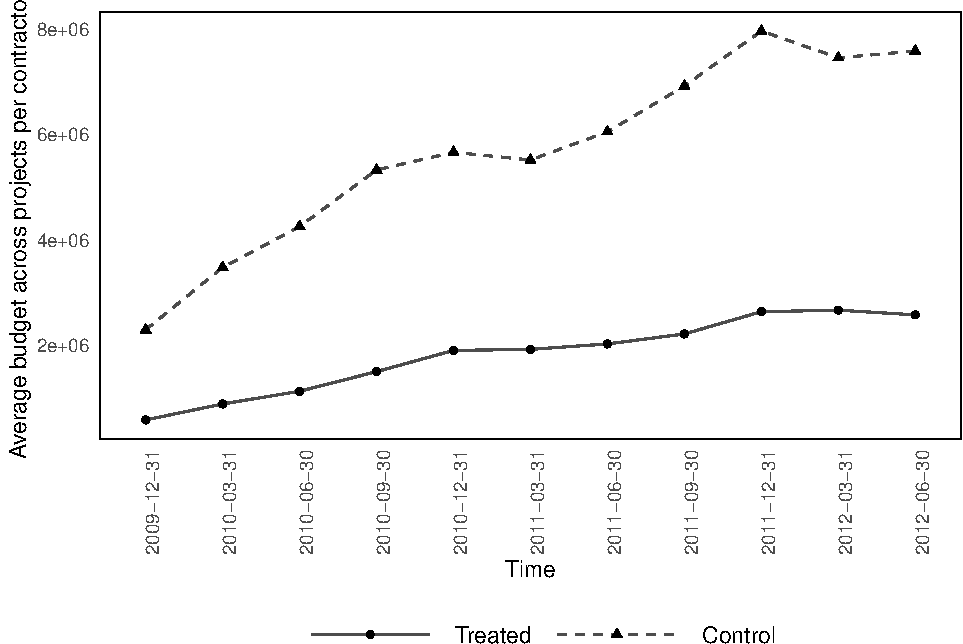
\includegraphics{qp_first_pc_delay_clean_control_time_independent_files/figure-latex/budget_0-1.pdf}

\begin{table}[H] \centering 
  \caption{Contractor Project Budget and QuickPay reform} 
  \label{} 
\small 
\begin{tabular}{@{\extracolsep{-2pt}}lcc} 
\\[-1.8ex]\hline 
\hline \\[-1.8ex] 
\\[-1.8ex] & \multicolumn{2}{c}{Total budget} \\ 
\\[-1.8ex] & (1) & (2)\\ 
\hline \\[-1.8ex] 
 $Treat_i$ & $-$3,303,977.00$^{***}$ & $-$3,296,074.00$^{***}$ \\ 
  & (525,130.10) & (527,240.20) \\ 
  & & \\ 
 $Post_t$ & 2,457,755.00$^{***}$ &  \\ 
  & (287,992.90) &  \\ 
  & & \\ 
 $Treat_i \times Post_t$ & $-$1,472,315.00$^{***}$ & $-$1,475,519.00$^{***}$ \\ 
  & (291,443.10) & (292,600.50) \\ 
  & & \\ 
 Constant & 4,733,618.00$^{***}$ &  \\ 
  & (522,700.30) &  \\ 
  & & \\ 
\hline \\[-1.8ex] 
Time fixed effects & No & Yes \\ 
Observations & 84,391 & 84,391 \\ 
R$^{2}$ & 0.02 & 0.02 \\ 
Adjusted R$^{2}$ & 0.02 & 0.02 \\ 
\hline 
\hline \\[-1.8ex] 
\textit{Note:}  & \multicolumn{2}{r}{$^{*}$p$<$0.1; $^{**}$p$<$0.05; $^{***}$p$<$0.01} \\ 
 & \multicolumn{2}{r}{Each observation is a contractor-quarter.} \\ 
 & \multicolumn{2}{r}{SEs are robust and clustered at the contractor level.} \\ 
 & \multicolumn{2}{r}{Sample restricted to contractors performing only one type of project.} \\ 
\end{tabular} 
\end{table}

\hypertarget{number-of-tasks}{%
\subsection{Number of tasks}\label{number-of-tasks}}

\hypertarget{contractors-holding-only-small-or-only-large-projects-2}{%
\subsubsection{Contractors holding only small or only large
projects}\label{contractors-holding-only-small-or-only-large-projects-2}}

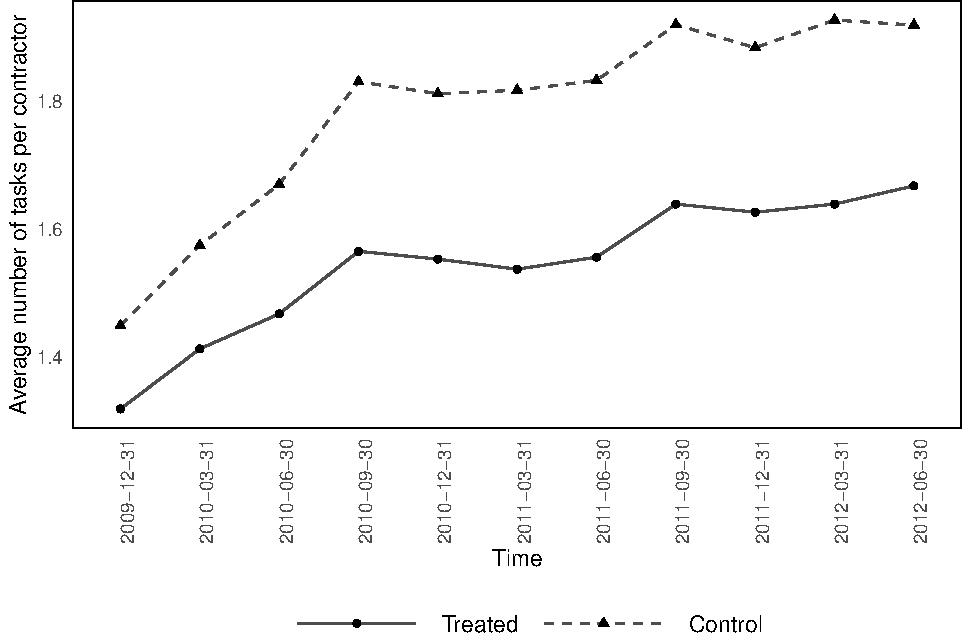
\includegraphics{qp_first_pc_delay_clean_control_time_independent_files/figure-latex/tasks_0-1.pdf}

\begin{table}[H] \centering 
  \caption{Contractor Project Tasks and QuickPay reform} 
  \label{} 
\small 
\begin{tabular}{@{\extracolsep{-2pt}}lcc} 
\\[-1.8ex]\hline 
\hline \\[-1.8ex] 
\\[-1.8ex] & \multicolumn{2}{c}{Number of tasks} \\ 
\\[-1.8ex] & (1) & (2)\\ 
\hline \\[-1.8ex] 
 $Treat_i$ & $-$0.23$^{***}$ & $-$0.23$^{***}$ \\ 
  & (0.04) & (0.04) \\ 
  & & \\ 
 $Post_t$ & 0.17$^{***}$ &  \\ 
  & (0.02) &  \\ 
  & & \\ 
 $Treat_i \times Post_t$ & $-$0.04 & $-$0.04 \\ 
  & (0.03) & (0.03) \\ 
  & & \\ 
 Constant & 1.73$^{***}$ &  \\ 
  & (0.04) &  \\ 
  & & \\ 
\hline \\[-1.8ex] 
Time fixed effects & No & Yes \\ 
Observations & 84,391 & 84,391 \\ 
R$^{2}$ & 0.01 & 0.01 \\ 
Adjusted R$^{2}$ & 0.01 & 0.01 \\ 
\hline 
\hline \\[-1.8ex] 
\textit{Note:}  & \multicolumn{2}{r}{$^{*}$p$<$0.1; $^{**}$p$<$0.05; $^{***}$p$<$0.01} \\ 
 & \multicolumn{2}{r}{Each observation is a contractor-quarter.} \\ 
 & \multicolumn{2}{r}{SEs are robust and clustered at the contractor level.} \\ 
 & \multicolumn{2}{r}{Sample restricted to contractors performing only one type of project.} \\ 
\end{tabular} 
\end{table}

\hypertarget{project-portfolio-spillover-effect}{%
\section{Project portfolio: Spillover
effect}\label{project-portfolio-spillover-effect}}

\hypertarget{regression-1-did-on-large-projects}{%
\subsection{Regression 1: DID on large
projects}\label{regression-1-did-on-large-projects}}

\begin{itemize}
\tightlist
\item
  Sample restricted to large projects only.
\item
  Treat is an indicator that equals one for LARGE projects whose
  contractor has at least one small project at any point, and is zero
  otherwise
\end{itemize}

\begin{table}[H] \centering 
  \caption{Project Portfolio and QuickPay reform} 
  \label{} 
\small 
\begin{tabular}{@{\extracolsep{-10pt}}lccccc} 
\\[-1.8ex]\hline 
\hline \\[-1.8ex] 
\\[-1.8ex] & \multicolumn{5}{c}{$PercentDelay_{it}$} \\ 
\\[-1.8ex] & (1) & (2) & (3) & (4) & (5)\\ 
\hline \\[-1.8ex] 
 $Treat_i$ & 1.53$^{***}$ & $-$0.55$^{***}$ & $-$0.64$^{***}$ & 0.43$^{**}$ & 0.46$^{***}$ \\ 
  & (0.23) & (0.17) & (0.17) & (0.17) & (0.17) \\ 
  & & & & & \\ 
 $Post_t$ & $-$0.35$^{***}$ & $-$13.73$^{***}$ &  &  &  \\ 
  & (0.13) & (1.19) &  &  &  \\ 
  & & & & & \\ 
 $Treat_i \times Post_t$ & 0.08 & 0.52$^{**}$ & 0.60$^{***}$ & 0.23 & 0.33 \\ 
  & (0.27) & (0.22) & (0.22) & (0.22) & (0.22) \\ 
  & & & & & \\ 
 Constant & 5.96$^{***}$ & 64.62$^{***}$ &  &  &  \\ 
  & (0.11) & (0.91) &  &  &  \\ 
  & & & & & \\ 
\hline \\[-1.8ex] 
Duration, Budget, Bids & No & Yes & Yes & Yes & Yes \\ 
$Post_t \times $  (Duration, Budget, Bids) & No & Yes & Yes & Yes & Yes \\ 
Project stage & No & Yes & Yes & Yes & Yes \\ 
Time fixed effects & No & No & Yes & Yes & Yes \\ 
Task fixed effects & No & No & No & Yes & Yes \\ 
Industry fixed effects & No & No & No & No & Yes \\ 
Observations & 117,787 & 110,601 & 110,601 & 110,601 & 110,601 \\ 
R$^{2}$ & 0.002 & 0.26 & 0.26 & 0.30 & 0.30 \\ 
Adjusted R$^{2}$ & 0.002 & 0.26 & 0.26 & 0.29 & 0.29 \\ 
\hline 
\hline \\[-1.8ex] 
\textit{Note:}  & \multicolumn{5}{r}{$^{*}$p$<$0.1; $^{**}$p$<$0.05; $^{***}$p$<$0.01} \\ 
 & \multicolumn{5}{r}{Each observation is a project-quarter.} \\ 
 & \multicolumn{5}{r}{SEs are robust and clustered at the project level.} \\ 
 & \multicolumn{5}{r}{Sample restricted to large projects only.} \\ 
\end{tabular} 
\end{table}

\hypertarget{regression-2-incremental-effect-on-small-project-with-existing-large-project}{%
\subsection{Regression 2: Incremental effect on small project with
existing large
project}\label{regression-2-incremental-effect-on-small-project-with-existing-large-project}}

\begin{itemize}
\tightlist
\item
  \(Treat_{i,l}\) is an indicator that equals 1 for small projects whose
  contractor holds a large project at any point in time, and is zero
  otherwise.
\item
  Large projects whose contractor holds small projects are removed to
  get a clean control group.
\end{itemize}

\begin{table}[H] \centering 
  \caption{(Incremental effect) Project Portfolio and QuickPay reform} 
  \label{} 
\small 
\begin{tabular}{@{\extracolsep{-2pt}}lccccc} 
\\[-1.8ex]\hline 
\hline \\[-1.8ex] 
\\[-1.8ex] & \multicolumn{5}{c}{$PercentDelay_{it}$  } \\ 
\\[-1.8ex] & (1) & (2) & (3) & (4) & (5)\\ 
\hline \\[-1.8ex] 
 $Treat_i$ & $-$0.79$^{***}$ & $-$0.48$^{***}$ & $-$0.54$^{***}$ & $-$0.68$^{***}$ & $-$0.71$^{***}$ \\ 
  & (0.13) & (0.11) & (0.11) & (0.12) & (0.12) \\ 
  & & & & & \\ 
 $Treat_{i,l}$ & $-$2.74$^{***}$ & $-$2.46$^{***}$ & $-$2.41$^{***}$ & $-$0.72$^{***}$ & $-$0.64$^{***}$ \\ 
  & (0.11) & (0.10) & (0.10) & (0.10) & (0.10) \\ 
  & & & & & \\ 
 $Post_t$ & $-$0.21$^{*}$ & $-$5.41$^{***}$ &  &  &  \\ 
  & (0.12) & (0.79) &  &  &  \\ 
  & & & & & \\ 
 $Treat_i \times Post_t$ & 1.22$^{***}$ & 1.04$^{***}$ & 1.09$^{***}$ & 1.11$^{***}$ & 1.13$^{***}$ \\ 
  & (0.15) & (0.15) & (0.15) & (0.15) & (0.15) \\ 
  & & & & & \\ 
 $Treat_{i,l} \times Post_t$ & $-$0.48$^{***}$ & $-$0.28$^{**}$ & $-$0.33$^{**}$ & $-$0.38$^{***}$ & $-$0.38$^{***}$ \\ 
  & (0.14) & (0.14) & (0.14) & (0.14) & (0.14) \\ 
  & & & & & \\ 
 Constant & 5.27$^{***}$ & 43.79$^{***}$ &  &  &  \\ 
  & (0.10) & (0.61) &  &  &  \\ 
  & & & & & \\ 
\hline \\[-1.8ex] 
Duration, Budget, Bids & No & Yes & Yes & Yes & Yes \\ 
$Post_t \times $  (Duration, Budget, Bids) & No & Yes & Yes & Yes & Yes \\ 
Project stage & No & Yes & Yes & Yes & Yes \\ 
Time fixed effects & No & No & Yes & Yes & Yes \\ 
Task fixed effects & No & No & No & Yes & Yes \\ 
Industry fixed effects & No & No & No & No & Yes \\ 
Observations & 223,244 & 201,738 & 201,738 & 201,738 & 201,738 \\ 
R$^{2}$ & 0.01 & 0.18 & 0.18 & 0.21 & 0.21 \\ 
Adjusted R$^{2}$ & 0.01 & 0.18 & 0.18 & 0.21 & 0.21 \\ 
\hline 
\hline \\[-1.8ex] 
\textit{Note:}  & \multicolumn{5}{r}{$^{*}$p$<$0.1; $^{**}$p$<$0.05; $^{***}$p$<$0.01} \\ 
 & \multicolumn{5}{r}{Each observation is a project-quarter.} \\ 
 & \multicolumn{5}{r}{SEs are robust and clustered at the project level.} \\ 
 & \multicolumn{5}{r}{Large projects whose contractor holds small projects are removed.} \\ 
\end{tabular} 
\end{table}

\hypertarget{project-stage}{%
\section{Project Stage}\label{project-stage}}

\begin{itemize}
\tightlist
\item
  \(t\) indicates the end of the quarter
\item
  We want to get stage of the project at the beginning of a given
  quarter (before any delays materialize)
\end{itemize}

\(Stage_{it}=\frac{ActionDate_{t-1}-StartDate_i}{Duration_{i,t-1}}\)
\(Stage_{it}=\frac{(t-1)-StartDate_i}{Duration_{i,t-1}}\)

\hypertarget{stage-quintile}{%
\subsection{Stage Quintile}\label{stage-quintile}}

\hypertarget{logged-stage-regressions}{%
\subsection{Logged Stage Regressions}\label{logged-stage-regressions}}

\begin{table}[H] \centering 
  \caption{Project Stage and QuickPay reform} 
  \label{} 
\small 
\begin{tabular}{@{\extracolsep{-2pt}}lccccc} 
\\[-1.8ex]\hline 
\hline \\[-1.8ex] 
\\[-1.8ex] & \multicolumn{5}{c}{$PercentDelay_{it}$  } \\ 
\\[-1.8ex] & (1) & (2) & (3) & (4) & (5)\\ 
\hline \\[-1.8ex] 
 $Treat_i$ & $-$2.65$^{***}$ & $-$1.65$^{***}$ & $-$1.73$^{***}$ & $-$1.34$^{***}$ & $-$1.37$^{***}$ \\ 
  & (0.23) & (0.21) & (0.21) & (0.21) & (0.20) \\ 
  & & & & & \\ 
 Log(Stage) & 3.16$^{***}$ & 2.51$^{***}$ & 2.45$^{***}$ & 2.53$^{***}$ & 2.53$^{***}$ \\ 
  & (0.08) & (0.07) & (0.07) & (0.07) & (0.07) \\ 
  & & & & & \\ 
 $Post_t$ & $-$1.33$^{***}$ & $-$5.06$^{***}$ &  &  &  \\ 
  & (0.23) & (0.81) &  &  &  \\ 
  & & & & & \\ 
 $Treat_i \times Post_t$ & 2.06$^{***}$ & 1.74$^{***}$ & 1.82$^{***}$ & 1.85$^{***}$ & 1.90$^{***}$ \\ 
  & (0.28) & (0.26) & (0.26) & (0.25) & (0.25) \\ 
  & & & & & \\ 
 $Treat_i \times$ Log(Stage) & $-$0.70$^{***}$ & $-$0.20$^{**}$ & $-$0.23$^{**}$ & $-$0.27$^{***}$ & $-$0.29$^{***}$ \\ 
  & (0.10) & (0.09) & (0.09) & (0.09) & (0.09) \\ 
  & & & & & \\ 
 $Post_t \times$ Log(Stage) & $-$0.06 & 0.48$^{***}$ & 0.49$^{***}$ & 0.23$^{**}$ & 0.22$^{**}$ \\ 
  & (0.10) & (0.09) & (0.09) & (0.09) & (0.09) \\ 
  & & & & & \\ 
 $Treat_i \times Post_t \times$ Log(Stage) & 0.59$^{***}$ & 0.54$^{***}$ & 0.56$^{***}$ & 0.62$^{***}$ & 0.63$^{***}$ \\ 
  & (0.12) & (0.11) & (0.11) & (0.11) & (0.11) \\ 
  & & & & & \\ 
 Constant & 10.20$^{***}$ & 43.10$^{***}$ &  &  &  \\ 
  & (0.19) & (0.62) &  &  &  \\ 
  & & & & & \\ 
\hline \\[-1.8ex] 
Duration, Budget, Bids & No & Yes & Yes & Yes & Yes \\ 
$Post_t \times $  (Duration, Budget, Bids) & No & Yes & Yes & Yes & Yes \\ 
Time fixed effects & No & No & Yes & Yes & Yes \\ 
Task fixed effects & No & No & No & Yes & Yes \\ 
Industry fixed effects & No & No & No & No & Yes \\ 
Observations & 223,213 & 201,738 & 201,738 & 201,738 & 201,738 \\ 
R$^{2}$ & 0.06 & 0.18 & 0.18 & 0.21 & 0.22 \\ 
Adjusted R$^{2}$ & 0.06 & 0.18 & 0.18 & 0.21 & 0.21 \\ 
\hline 
\hline \\[-1.8ex] 
\textit{Note:}  & \multicolumn{5}{r}{$^{*}$p$<$0.1; $^{**}$p$<$0.05; $^{***}$p$<$0.01} \\ 
 & \multicolumn{5}{r}{Each observation is a project-quarter.} \\ 
 & \multicolumn{5}{r}{SEs are robust and clustered at the project level.} \\ 
\end{tabular} 
\end{table}

\hypertarget{contract-financing-projects-active-onbefore-june-2010}{%
\section{Contract Financing (Projects active on/before June
2010)}\label{contract-financing-projects-active-onbefore-june-2010}}

\begin{itemize}
\tightlist
\item
  \(CF=1\) if project was receiving contract financing
\item
  Sample restricted to projects that started on or before June 2010
\item
  Jobs act was launched in Sept 2010
\end{itemize}

\begin{table}[H] \centering 
  \caption{Contract Financing and QuickPay reform} 
  \label{} 
\small 
\begin{tabular}{@{\extracolsep{-2pt}}lccccc} 
\\[-1.8ex]\hline 
\hline \\[-1.8ex] 
\\[-1.8ex] & \multicolumn{5}{c}{$PercentDelay_{it}$  } \\ 
\\[-1.8ex] & (1) & (2) & (3) & (4) & (5)\\ 
\hline \\[-1.8ex] 
 $Treat_i$ & $-$2.11$^{***}$ & $-$1.19$^{***}$ & $-$1.31$^{***}$ & $-$0.67$^{***}$ & $-$0.71$^{***}$ \\ 
  & (0.16) & (0.15) & (0.15) & (0.16) & (0.16) \\ 
  & & & & & \\ 
 $Post_t$ & 1.44$^{***}$ & $-$8.73$^{***}$ &  &  &  \\ 
  & (0.28) & (2.64) &  &  &  \\ 
  & & & & & \\ 
 $CF_i$ & 1.32$^{***}$ & 1.64$^{***}$ & 1.40$^{***}$ & $-$0.56 & $-$0.64$^{*}$ \\ 
  & (0.37) & (0.32) & (0.31) & (0.34) & (0.34) \\ 
  & & & & & \\ 
 $Treat_i \times Post_t$ & $-$0.03 & 2.35$^{***}$ & 2.46$^{***}$ & 2.40$^{***}$ & 2.43$^{***}$ \\ 
  & (0.33) & (0.43) & (0.43) & (0.45) & (0.45) \\ 
  & & & & & \\ 
 $Post_t \times CF_i$ & 0.04 & $-$1.30$^{**}$ & $-$1.07 & 0.39 & 0.44 \\ 
  & (0.65) & (0.66) & (0.65) & (0.68) & (0.68) \\ 
  & & & & & \\ 
 $Treat_i \times CF_i$ & 1.98$^{***}$ & 1.00$^{**}$ & 1.05$^{***}$ & 0.60 & 0.59 \\ 
  & (0.48) & (0.41) & (0.40) & (0.42) & (0.42) \\ 
  & & & & & \\ 
 $Treat_i \times Post_t \times CF_i$ & 0.77 & $-$1.40 & $-$1.44 & $-$0.81 & $-$0.88 \\ 
  & (0.89) & (0.90) & (0.89) & (0.92) & (0.92) \\ 
  & & & & & \\ 
 Constant & 5.33$^{***}$ & 46.80$^{***}$ &  &  &  \\ 
  & (0.14) & (0.84) &  &  &  \\ 
  & & & & & \\ 
\hline \\[-1.8ex] 
Duration, Budget, Bids & No & Yes & Yes & Yes & Yes \\ 
$Post_t \times $  (Duration, Budget, Bids) & No & Yes & Yes & Yes & Yes \\ 
Project stage & No & Yes & Yes & Yes & Yes \\ 
Time fixed effects & No & No & Yes & Yes & Yes \\ 
Task fixed effects & No & No & No & Yes & Yes \\ 
Industry fixed effects & No & No & No & No & Yes \\ 
Observations & 65,191 & 55,291 & 55,291 & 55,291 & 55,291 \\ 
R$^{2}$ & 0.01 & 0.18 & 0.18 & 0.23 & 0.23 \\ 
Adjusted R$^{2}$ & 0.01 & 0.18 & 0.18 & 0.22 & 0.22 \\ 
\hline 
\hline \\[-1.8ex] 
\textit{Note:}  & \multicolumn{5}{r}{$^{*}$p$<$0.1; $^{**}$p$<$0.05; $^{***}$p$<$0.01} \\ 
 & \multicolumn{5}{r}{Each observation is a project-quarter.} \\ 
 & \multicolumn{5}{r}{SEs are robust and clustered at the project level.} \\ 
\end{tabular} 
\end{table}

\hypertarget{competition}{%
\section{Competition}\label{competition}}

\hypertarget{impact-on-bidding-metrics-all-projects}{%
\subsection{Impact on bidding metrics {[}All
projects{]}}\label{impact-on-bidding-metrics-all-projects}}

\begin{table}[H] \centering 
  \caption{Effect of Competition After QuickPay: Quickpay 2009-2011} 
  \label{} 
\small 
\begin{tabular}{@{\extracolsep{0pt}}lccc} 
\\[-1.8ex]\hline 
\hline \\[-1.8ex] 
\\[-1.8ex] & $NumberOfBids_{it}$ & $InitialDuration_{it}$ & $InitialBudget_{it}$ \\ 
\\[-1.8ex] & (1) & (2) & (3)\\ 
\hline \\[-1.8ex] 
 $Treat_i$ & 1.08$^{***}$ & $-$7.27$^{***}$ & $-$15,055.20$^{***}$ \\ 
  & (0.02) & (0.72) & (1,586.13) \\ 
  & & & \\ 
 $Treat_i \times Post_t$ & 0.09$^{***}$ & $-$3.38$^{***}$ & $-$29,491.30$^{***}$ \\ 
  & (0.03) & (1.00) & (2,296.49) \\ 
  & & & \\ 
\hline \\[-1.8ex] 
Task fixed effects & Yes & Yes & Yes \\ 
Time fixed effects & Yes & Yes & Yes \\ 
Observations & 227,609 & 220,550 & 227,732 \\ 
R$^{2}$ & 0.20 & 0.20 & 0.24 \\ 
Adjusted R$^{2}$ & 0.19 & 0.19 & 0.24 \\ 
\hline 
\hline \\[-1.8ex] 
\textit{Note:}  & \multicolumn{3}{r}{$^{*}$p$<$0.1; $^{**}$p$<$0.05; $^{***}$p$<$0.01} \\ 
 & \multicolumn{3}{r}{Each observation is a project-quarter.} \\ 
 & \multicolumn{3}{r}{SEs are robust and clustered at the project level.} \\ 
 & \multicolumn{3}{r}{Sample restricted to fully competed projects.} \\ 
\end{tabular} 
\end{table}

\hypertarget{impact-on-delays}{%
\subsection{Impact on delays}\label{impact-on-delays}}

\hypertarget{subsample-model-ii}{%
\subsubsection{Subsample model II}\label{subsample-model-ii}}

Define
\[ SA_i = \begin{cases} 1, \text{ if project was signed after QuickPay}\\
0, \text{ otherwise} \end{cases}\]

\[ SB_i = \begin{cases} 1, \text{ if project was signed before QuickPay}\\
0, \text{ otherwise} \end{cases}\]

\begin{table}[H] \centering 
  \caption{Effect of QuickPay on competitively awarded projects} 
  \label{} 
\small 
\begin{tabular}{@{\extracolsep{-2pt}}lccccc} 
\\[-1.8ex]\hline 
\hline \\[-1.8ex] 
\\[-1.8ex] & \multicolumn{5}{c}{$PercentDelay_{it}$  } \\ 
\\[-1.8ex] & (1) & (2) & (3) & (4) & (5)\\ 
\hline \\[-1.8ex] 
 $Treat_i$ & $-$2.26$^{***}$ & $-$1.93$^{***}$ & $-$1.94$^{***}$ & $-$0.50$^{***}$ & $-$0.51$^{***}$ \\ 
  & (0.13) & (0.12) & (0.12) & (0.12) & (0.12) \\ 
  & & & & & \\ 
 $SA_i$ & $-$1.90$^{***}$ & 0.87$^{***}$ & 1.45$^{***}$ & 1.52$^{***}$ & 1.48$^{***}$ \\ 
  & (0.17) & (0.16) & (0.18) & (0.18) & (0.18) \\ 
  & & & & & \\ 
 $Post_t$ & 1.18$^{***}$ & $-$1.16$^{***}$ &  &  &  \\ 
  & (0.16) & (0.16) &  &  &  \\ 
  & & & & & \\ 
 $Treat_i \times Post_t$ & 0.23 & 0.28 & 0.30$^{*}$ & 0.16 & 0.16 \\ 
  & (0.19) & (0.18) & (0.18) & (0.17) & (0.17) \\ 
  & & & & & \\ 
 $Treat_i \times Post_t \times SA_i $ & 0.98$^{***}$ & 0.60$^{***}$ & 0.58$^{***}$ & 0.76$^{***}$ & 0.76$^{***}$ \\ 
  & (0.20) & (0.19) & (0.19) & (0.19) & (0.19) \\ 
  & & & & & \\ 
 Constant & 5.48$^{***}$ & 10.06$^{***}$ &  &  &  \\ 
  & (0.11) & (0.13) &  &  &  \\ 
  & & & & & \\ 
\hline \\[-1.8ex] 
Project stage & No & Yes & Yes & Yes & Yes \\ 
Time fixed effects & No & No & Yes & Yes & Yes \\ 
Task fixed effects & No & No & No & Yes & Yes \\ 
Industry fixed effects & No & No & No & No & Yes \\ 
Observations & 184,911 & 184,885 & 184,885 & 184,885 & 184,885 \\ 
R$^{2}$ & 0.01 & 0.06 & 0.06 & 0.12 & 0.13 \\ 
Adjusted R$^{2}$ & 0.01 & 0.06 & 0.06 & 0.12 & 0.12 \\ 
\hline 
\hline \\[-1.8ex] 
\textit{Note:}  & \multicolumn{5}{r}{$^{*}$p$<$0.1; $^{**}$p$<$0.05; $^{***}$p$<$0.01} \\ 
 & \multicolumn{5}{r}{Each observation is a project-quarter.} \\ 
 & \multicolumn{5}{r}{SEs are robust and clustered at the project level.} \\ 
 & \multicolumn{5}{r}{Sample restricted to fully competed projects.} \\ 
\end{tabular} 
\end{table}

\begin{table}[H] \centering 
  \caption{Effect of QuickPay on non-competitively awarded projects} 
  \label{} 
\small 
\begin{tabular}{@{\extracolsep{-2pt}}lccccc} 
\\[-1.8ex]\hline 
\hline \\[-1.8ex] 
\\[-1.8ex] & \multicolumn{5}{c}{$PercentDelay_{it}$  } \\ 
\\[-1.8ex] & (1) & (2) & (3) & (4) & (5)\\ 
\hline \\[-1.8ex] 
 $Treat_i$ & 1.16$^{***}$ & 0.96$^{***}$ & 0.89$^{***}$ & $-$0.17 & $-$0.11 \\ 
  & (0.28) & (0.27) & (0.27) & (0.29) & (0.28) \\ 
  & & & & & \\ 
 $SA_i$ & $-$0.61$^{***}$ & 1.94$^{***}$ & 3.19$^{***}$ & 2.82$^{***}$ & 2.74$^{***}$ \\ 
  & (0.22) & (0.22) & (0.26) & (0.26) & (0.26) \\ 
  & & & & & \\ 
 $Post_t$ & $-$0.79$^{***}$ & $-$3.11$^{***}$ &  &  &  \\ 
  & (0.24) & (0.25) &  &  &  \\ 
  & & & & & \\ 
 $Treat_i \times Post_t$ & 2.69$^{***}$ & 2.44$^{***}$ & 2.34$^{***}$ & 1.85$^{***}$ & 1.76$^{***}$ \\ 
  & (0.40) & (0.38) & (0.39) & (0.38) & (0.39) \\ 
  & & & & & \\ 
 $Treat_i \times Post_t \times SA_i $ & $-$1.89$^{***}$ & $-$1.67$^{***}$ & $-$1.63$^{***}$ & $-$1.87$^{***}$ & $-$1.75$^{***}$ \\ 
  & (0.39) & (0.37) & (0.37) & (0.37) & (0.37) \\ 
  & & & & & \\ 
 Constant & 4.40$^{***}$ & 9.65$^{***}$ &  &  &  \\ 
  & (0.20) & (0.25) &  &  &  \\ 
  & & & & & \\ 
\hline \\[-1.8ex] 
Project stage & No & Yes & Yes & Yes & Yes \\ 
Time fixed effects & No & No & Yes & Yes & Yes \\ 
Task fixed effects & No & No & No & Yes & Yes \\ 
Industry fixed effects & No & No & No & No & Yes \\ 
Observations & 38,175 & 38,170 & 38,170 & 38,170 & 38,170 \\ 
R$^{2}$ & 0.01 & 0.06 & 0.07 & 0.15 & 0.15 \\ 
Adjusted R$^{2}$ & 0.01 & 0.06 & 0.07 & 0.13 & 0.13 \\ 
\hline 
\hline \\[-1.8ex] 
\textit{Note:}  & \multicolumn{5}{r}{$^{*}$p$<$0.1; $^{**}$p$<$0.05; $^{***}$p$<$0.01} \\ 
 & \multicolumn{5}{r}{Each observation is a project-quarter.} \\ 
 & \multicolumn{5}{r}{SEs are robust and clustered at the project level.} \\ 
 & \multicolumn{5}{r}{Sample restricted to non-competed projects.} \\ 
\end{tabular} 
\end{table}

\hypertarget{four-way-interaction}{%
\subsubsection{Four-way interaction}\label{four-way-interaction}}

We run the following model:

\[\begin{aligned} PercentDelay_{it} &=& \beta_0 +\beta_1 Treat_i+ \beta_2 StartedAfterQP_i+ \beta_3 Post_t+ \beta_4 Competitive_i\\ && +  \beta_5 (Treat_i \times Competitive_i) + \beta_6 (Post_t \times Competitive_i)\\ && +  \beta_7 (StartedAfterQP_i \times Competitive_i) +\beta_8 (Treat_i \times Post_t)\\ && + \beta_9 (Treat_i \times Post_t \times Competitive_i) \\ && + \beta_{10} (Treat_i \times Post_t \times StartedAfterQP_i )\\ && + \beta_{11} (Treat_i \times Post_t \times StartedAfterQP_i \times Competitive_i) + e_{it} \end{aligned}\]

\textbf{Interpretation:}

\begin{itemize}
\tightlist
\item
  \(\beta_9\) is the difference between treatment effect for competitive
  and non-competitive projects signed before quickpay.
\item
  \(\beta_9 + \beta_{11}\) is the difference between treatment effect
  for competitive and non-competitive projects signed \emph{after}
  quickpay.
\item
  \(\beta_{11}\) is our coefficient of interest because it tells us how
  much of the difference is there due to ``aggressive bidding'' after
  the policy.
\end{itemize}

\begin{table}[H] \centering 
  \caption{Effect of Competition After QuickPay: Quickpay 2009-2011} 
  \label{} 
\small 
\begin{tabular}{@{\extracolsep{-3pt}}lcccccc} 
\\[-1.8ex]\hline 
\hline \\[-1.8ex] 
\\[-1.8ex] & \multicolumn{6}{c}{$PercentDelay_{it}$  } \\ 
\\[-1.8ex] & (1) & (2) & (3) & (4) & (5) & (6)\\ 
\hline \\[-1.8ex] 
 $Treat_i$ & 1.16$^{***}$ & 1.16$^{***}$ & 0.97$^{***}$ & 0.92$^{***}$ & $-$0.26 & $-$0.28 \\ 
  & (0.28) & (0.28) & (0.27) & (0.27) & (0.27) & (0.27) \\ 
  & & & & & & \\ 
 $SA_i$ & $-$0.61$^{***}$ & $-$0.61$^{***}$ & 1.79$^{***}$ & 2.50$^{***}$ & 2.32$^{***}$ & 2.26$^{***}$ \\ 
  & (0.22) & (0.22) & (0.21) & (0.22) & (0.21) & (0.21) \\ 
  & & & & & & \\ 
 $Competitive_i$ & 1.08$^{***}$ & 1.08$^{***}$ & 0.79$^{***}$ & 0.77$^{***}$ & $-$0.74$^{***}$ & $-$0.69$^{***}$ \\ 
  & (0.23) & (0.23) & (0.22) & (0.22) & (0.23) & (0.23) \\ 
  & & & & & & \\ 
 $Post_t$ & $-$0.79$^{***}$ & $-$0.79$^{***}$ & $-$2.97$^{***}$ &  &  &  \\ 
  & (0.24) & (0.24) & (0.24) &  &  &  \\ 
  & & & & & & \\ 
 $Treat_i \times Competitive_i$ & $-$3.42$^{***}$ & $-$3.42$^{***}$ & $-$2.90$^{***}$ & $-$2.85$^{***}$ & $-$0.27 & $-$0.25 \\ 
  & (0.31) & (0.31) & (0.29) & (0.29) & (0.30) & (0.30) \\ 
  & & & & & & \\ 
 $Post_t \times Competitive_i$ & 1.97$^{***}$ & 1.97$^{***}$ & 1.78$^{***}$ & 1.74$^{***}$ & 0.73$^{***}$ & 0.64$^{**}$ \\ 
  & (0.29) & (0.29) & (0.28) & (0.28) & (0.28) & (0.28) \\ 
  & & & & & & \\ 
 $SA_i \times Competitive_i$ & $-$1.29$^{***}$ & $-$1.29$^{***}$ & $-$0.88$^{***}$ & $-$0.89$^{***}$ & $-$0.72$^{***}$ & $-$0.71$^{***}$ \\ 
  & (0.28) & (0.28) & (0.26) & (0.26) & (0.26) & (0.26) \\ 
  & & & & & & \\ 
 $Treat_i \times Post_t$ & 2.69$^{***}$ & 2.69$^{***}$ & 2.45$^{***}$ & 2.42$^{***}$ & 1.66$^{***}$ & 1.59$^{***}$ \\ 
  & (0.40) & (0.40) & (0.38) & (0.38) & (0.38) & (0.38) \\ 
  & & & & & & \\ 
 $Treat_i \times Post_t \times Competitive_i$ & $-$2.45$^{***}$ & $-$2.45$^{***}$ & $-$2.17$^{***}$ & $-$2.13$^{***}$ & $-$1.48$^{***}$ & $-$1.41$^{***}$ \\ 
  & (0.44) & (0.44) & (0.42) & (0.42) & (0.42) & (0.42) \\ 
  & & & & & & \\ 
 $Treat_i \times Post_t \times SA_i$ & $-$1.89$^{***}$ & $-$1.89$^{***}$ & $-$1.68$^{***}$ & $-$1.68$^{***}$ & $-$1.44$^{***}$ & $-$1.44$^{***}$ \\ 
  & (0.39) & (0.39) & (0.37) & (0.37) & (0.36) & (0.36) \\ 
  & & & & & & \\ 
 $Treat_i \times Post_t \times SA_i \times Competitive_i$ & 2.87$^{***}$ & 2.87$^{***}$ & 2.28$^{***}$ & 2.25$^{***}$ & 2.19$^{***}$ & 2.21$^{***}$ \\ 
  & (0.44) & (0.44) & (0.42) & (0.42) & (0.41) & (0.41) \\ 
  & & & & & & \\ 
 Constant & 4.40$^{***}$ & 4.40$^{***}$ & 9.33$^{***}$ &  &  &  \\ 
  & (0.20) & (0.20) & (0.20) &  &  &  \\ 
  & & & & & & \\ 
\hline \\[-1.8ex] 
Project stage & No & No & Yes & Yes & Yes & Yes \\ 
Time fixed effects & No & No & No & Yes & Yes & Yes \\ 
Task fixed effects & No & No & No & No & Yes & Yes \\ 
Industry fixed effects & No & No & No & No & No & Yes \\ 
Observations & 223,086 & 223,086 & 223,055 & 223,055 & 223,055 & 223,055 \\ 
R$^{2}$ & 0.01 & 0.01 & 0.06 & 0.06 & 0.12 & 0.12 \\ 
Adjusted R$^{2}$ & 0.01 & 0.01 & 0.06 & 0.06 & 0.11 & 0.12 \\ 
\hline 
\hline \\[-1.8ex] 
\textit{Note:}  & \multicolumn{6}{r}{$^{*}$p$<$0.1; $^{**}$p$<$0.05; $^{***}$p$<$0.01} \\ 
 & \multicolumn{6}{r}{Each observation is a project-quarter.} \\ 
 & \multicolumn{6}{r}{SEs are robust and clustered at the project level.} \\ 
\end{tabular} 
\end{table}

\end{document}
